\documentclass[aspectratio=169,11pt]{beamer}
\usepackage{iftex}
\ifPDFTeX
  \usepackage[utf8]{inputenc}
  \usepackage[T1]{fontenc}
\fi
\usepackage[brazil]{babel}
\usepackage{graphicx}
\usepackage{booktabs}
\usepackage{amsmath}

% ---- tema / cores ----
\usetheme{Madrid}
\usecolortheme{seahorse}
\definecolor{aptxblue}{RGB}{30,60,110}
\definecolor{aptxred}{RGB}{178,34,52}
\definecolor{aptxgreen}{RGB}{34,120,60}
\setbeamercolor{structure}{fg=aptxblue}
\setbeamercolor{frametitle}{bg=aptxblue,fg=white}
\setbeamertemplate{navigation symbols}{}
\setbeamertemplate{footline}[frame number]
\setbeamerfont{frametitle}{size=\large,series=\bfseries}
\newcommand{\gene}[1]{\textit{#1}}
\setbeamertemplate{itemize items}[circle]

\title[Redes gênicas e a perda de APTX]{Redes gênicas e a perda de \gene{APTX} (AOA1)}
\subtitle{Reprogramação do transcriptoma e o módulo das ataxias de reparo de DNA}
\author[P. H. R. Prado]{Pedro Henrique Ramos Prado, MSc.}
\institute[UFPR/PPGInf]{Programa de Pós-Graduação em Informática (PPGInf)\\Universidade Federal do Paraná}
\date{Biologia de Sistemas - 2026}

\begin{document}

% ---------- Slide 1: título ----------
\begin{frame}[plain]
  \titlepage
  \begin{center}\footnotesize\textcolor{aptxblue}{Reanálise de dados públicos (GEO GSE245766) com métodos de Biologia de Sistemas}\end{center}
\end{frame}

% ---------- Slide 2: motivação ----------
\begin{frame}{O problema: uma enzima de reparo de DNA no sistema imune}
  \begin{columns}[T]
    \begin{column}{0.56\textwidth}
      \begin{itemize}
        \item A \gene{APTX} (aprataxina) \textbf{repara quebras de fita simples de DNA}; sua perda causa a \textbf{Ataxia com Apraxia Oculomotora tipo 1 (AOA1)}.
        \item \textbf{Pergunta:} como a perda de \gene{APTX} reorganiza o transcriptoma da microglia humana?
        \item \textbf{Surpresa central:} o efeito dominante não está no reparo de DNA, mas no \textcolor{aptxred}{\textbf{programa de interferon}} (defesa antiviral).
      \end{itemize}
    \end{column}
    \begin{column}{0.44\textwidth}
      \small
      \begin{block}{Eixo interferon}
        Sensores de DNA/RNA (cGAS--STING, RIG-I) $\rightarrow$ interferon $\rightarrow$ centenas de \emph{genes estimulados por interferon} (ISGs: \gene{IFI44L}, \gene{OAS1}, \gene{MX1}\ldots).
      \end{block}
      \begin{alertblock}{Hipótese do estudo}
        O reparo de DNA e o alarme antiviral estão acoplados - e a \gene{APTX} é necessária para manter esse alarme.
      \end{alertblock}
    \end{column}
  \end{columns}
\end{frame}

% ---------- Slide 3: dados e pipeline ----------
\begin{frame}{Dados e desenho analítico}
  \begin{columns}[c]
    \begin{column}{0.40\textwidth}
      \small
      \begin{itemize}
        \item \textbf{GSE245766} (público): microglia HMC3.
        \item Desenho \textbf{2$\times$2 fatorial}: genótipo (\gene{APTX}-KO vs.\ WT) $\times$ estímulo imune (IS vs.\ NS), $n=12$.
        \item \textbf{15\,470 genes} após filtragem (log-CPM).
        \item Pipeline: DESeq2 $\rightarrow$ discretização/booleano $\rightarrow$ inferência de rede $\rightarrow$ validação contra STRING.
      \end{itemize}
      \begin{block}{KO funcional}
        \gene{APTX} não está reduzida no mRNA ($\log_2\mathrm{FC}=+0{,}21$): é \textbf{perda de função}, não de expressão.
      \end{block}
    \end{column}
    \begin{column}{0.60\textwidth}
      \centering
      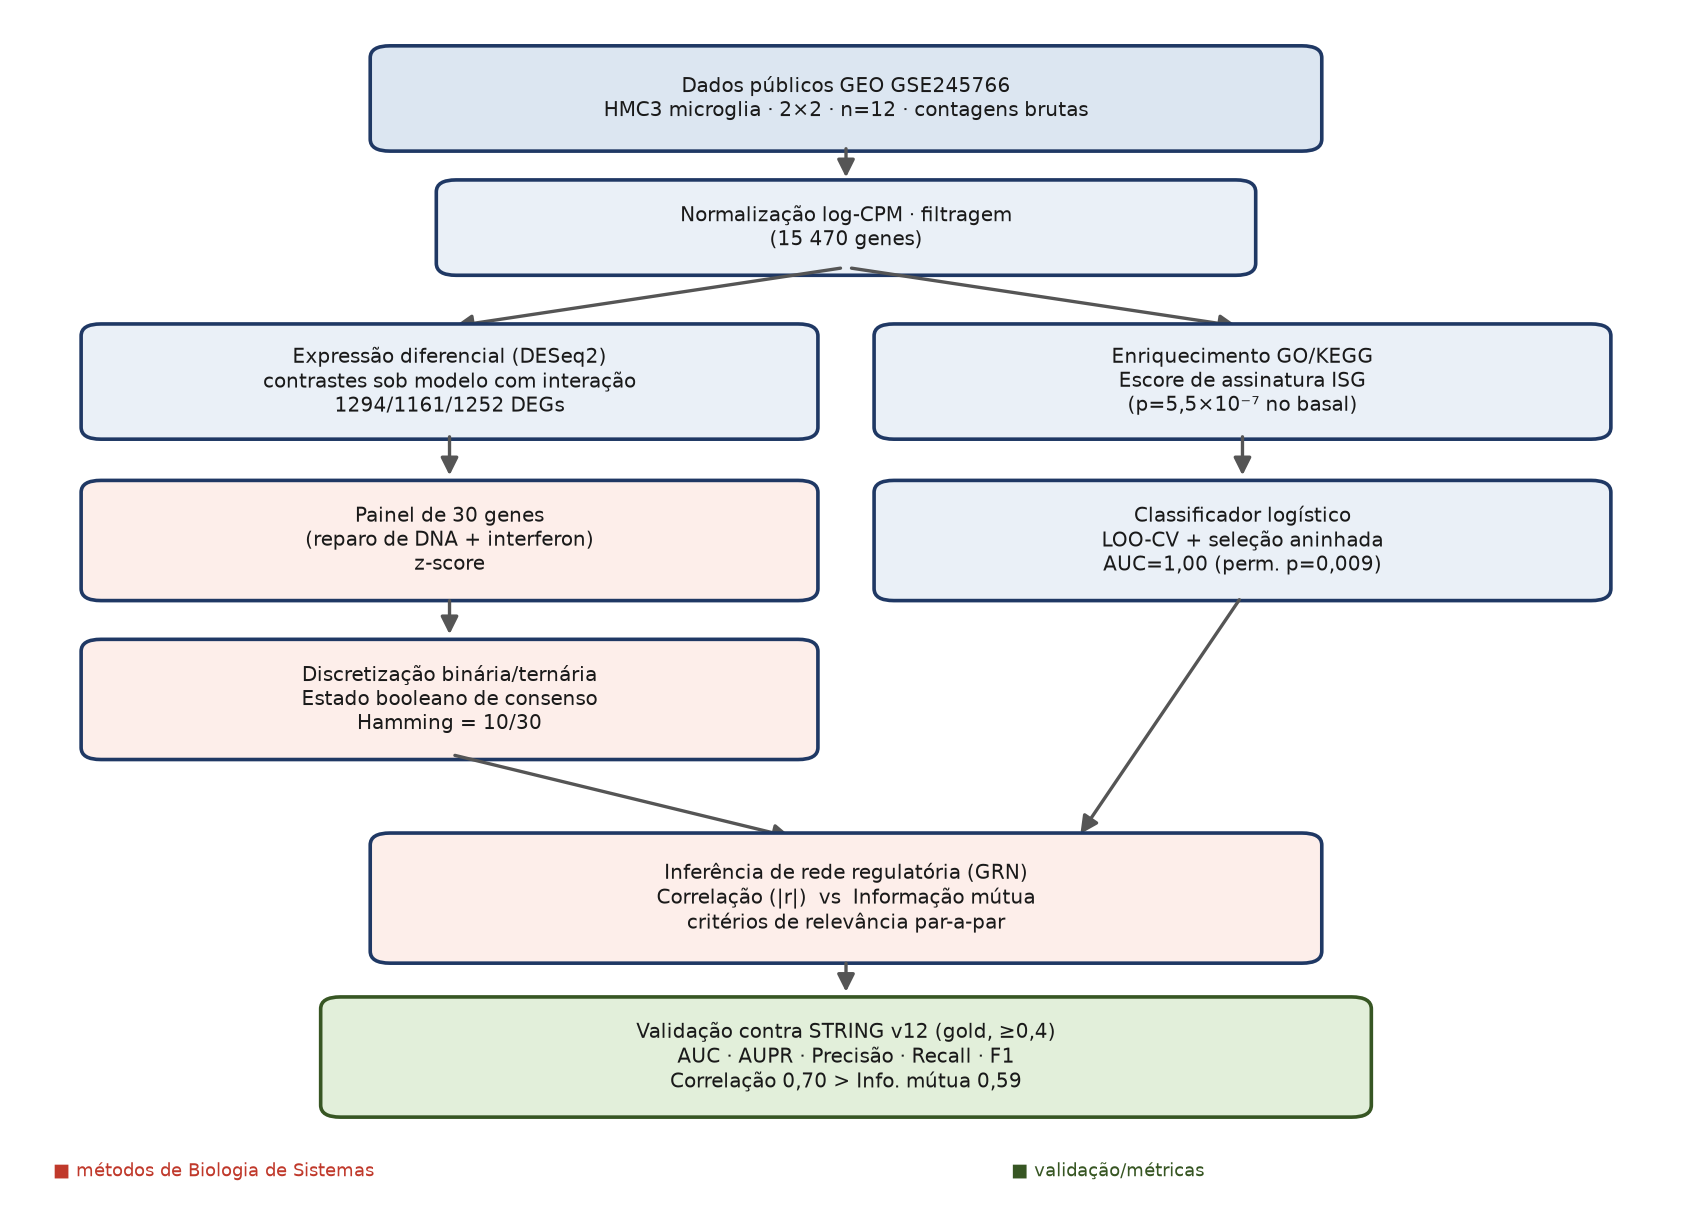
\includegraphics[width=\textwidth,height=0.82\textheight,keepaspectratio]{figure_fluxograma.png}
    \end{column}
  \end{columns}
\end{frame}

% ---------- Slide 4: resultado biológico ----------
\begin{frame}{Resultado 1 - programa de interferon reprimido no KO}
  \centering
  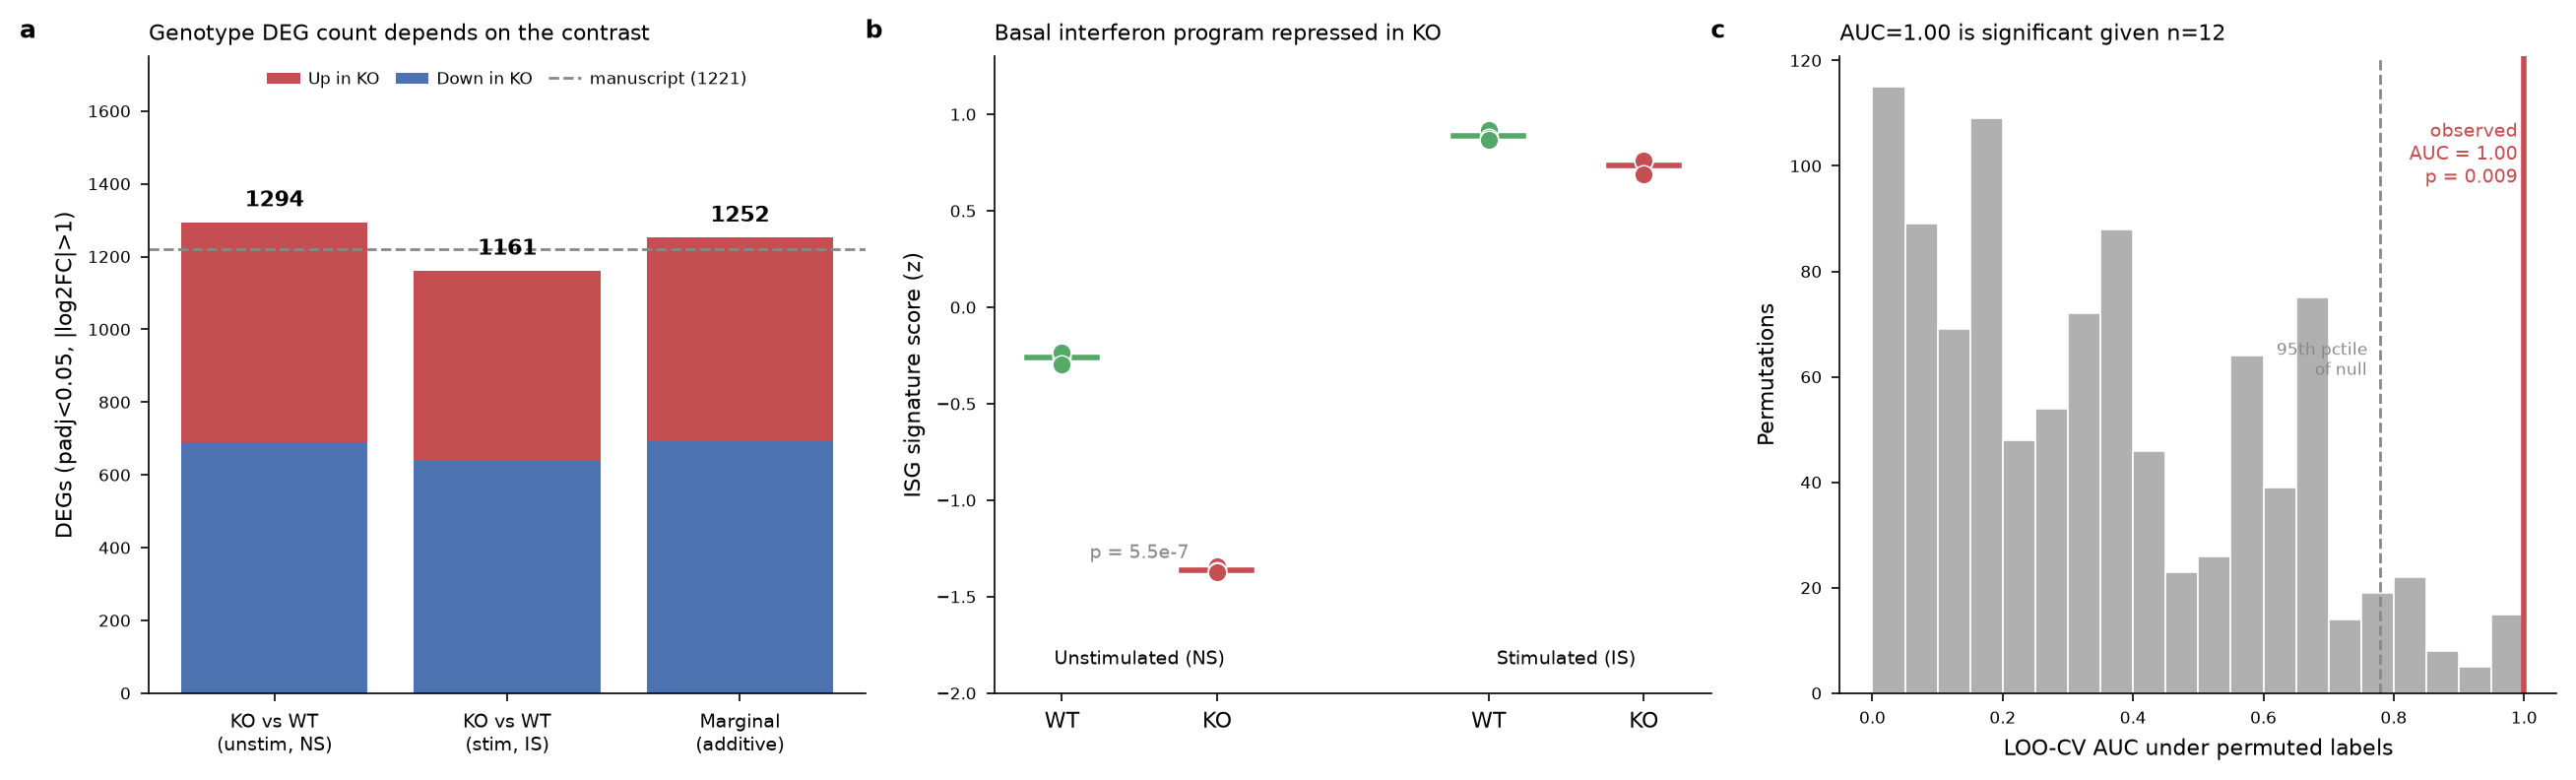
\includegraphics[width=\textwidth,height=0.70\textheight,keepaspectratio]{figure_reanalysis.png}
  \vspace{0.3em}
  \begin{columns}
    \begin{column}{0.94\textwidth}\small
      \textbf{(a)} $\sim$1\,300 DEGs de genótipo (reproduz o artigo original). \quad
      \textbf{(b)} Escore ISG \textbf{fortemente reprimido no KO no basal} (NS: $-1{,}36$ vs.\ $-0{,}26$; $p=5{,}5\times10^{-7}$). \quad
      \textbf{(c)} O classificador (AUC$=$1,00) é significativo mesmo com $n=12$ (permutação, $p=0{,}009$).
    \end{column}
  \end{columns}
\end{frame}

% ---------- Slide 5: métodos de biologia de sistemas ----------
\begin{frame}{Métodos de Biologia de Sistemas - discretização e rede booleana}
  \begin{columns}[c]
    \begin{column}{0.60\textwidth}
      \centering
      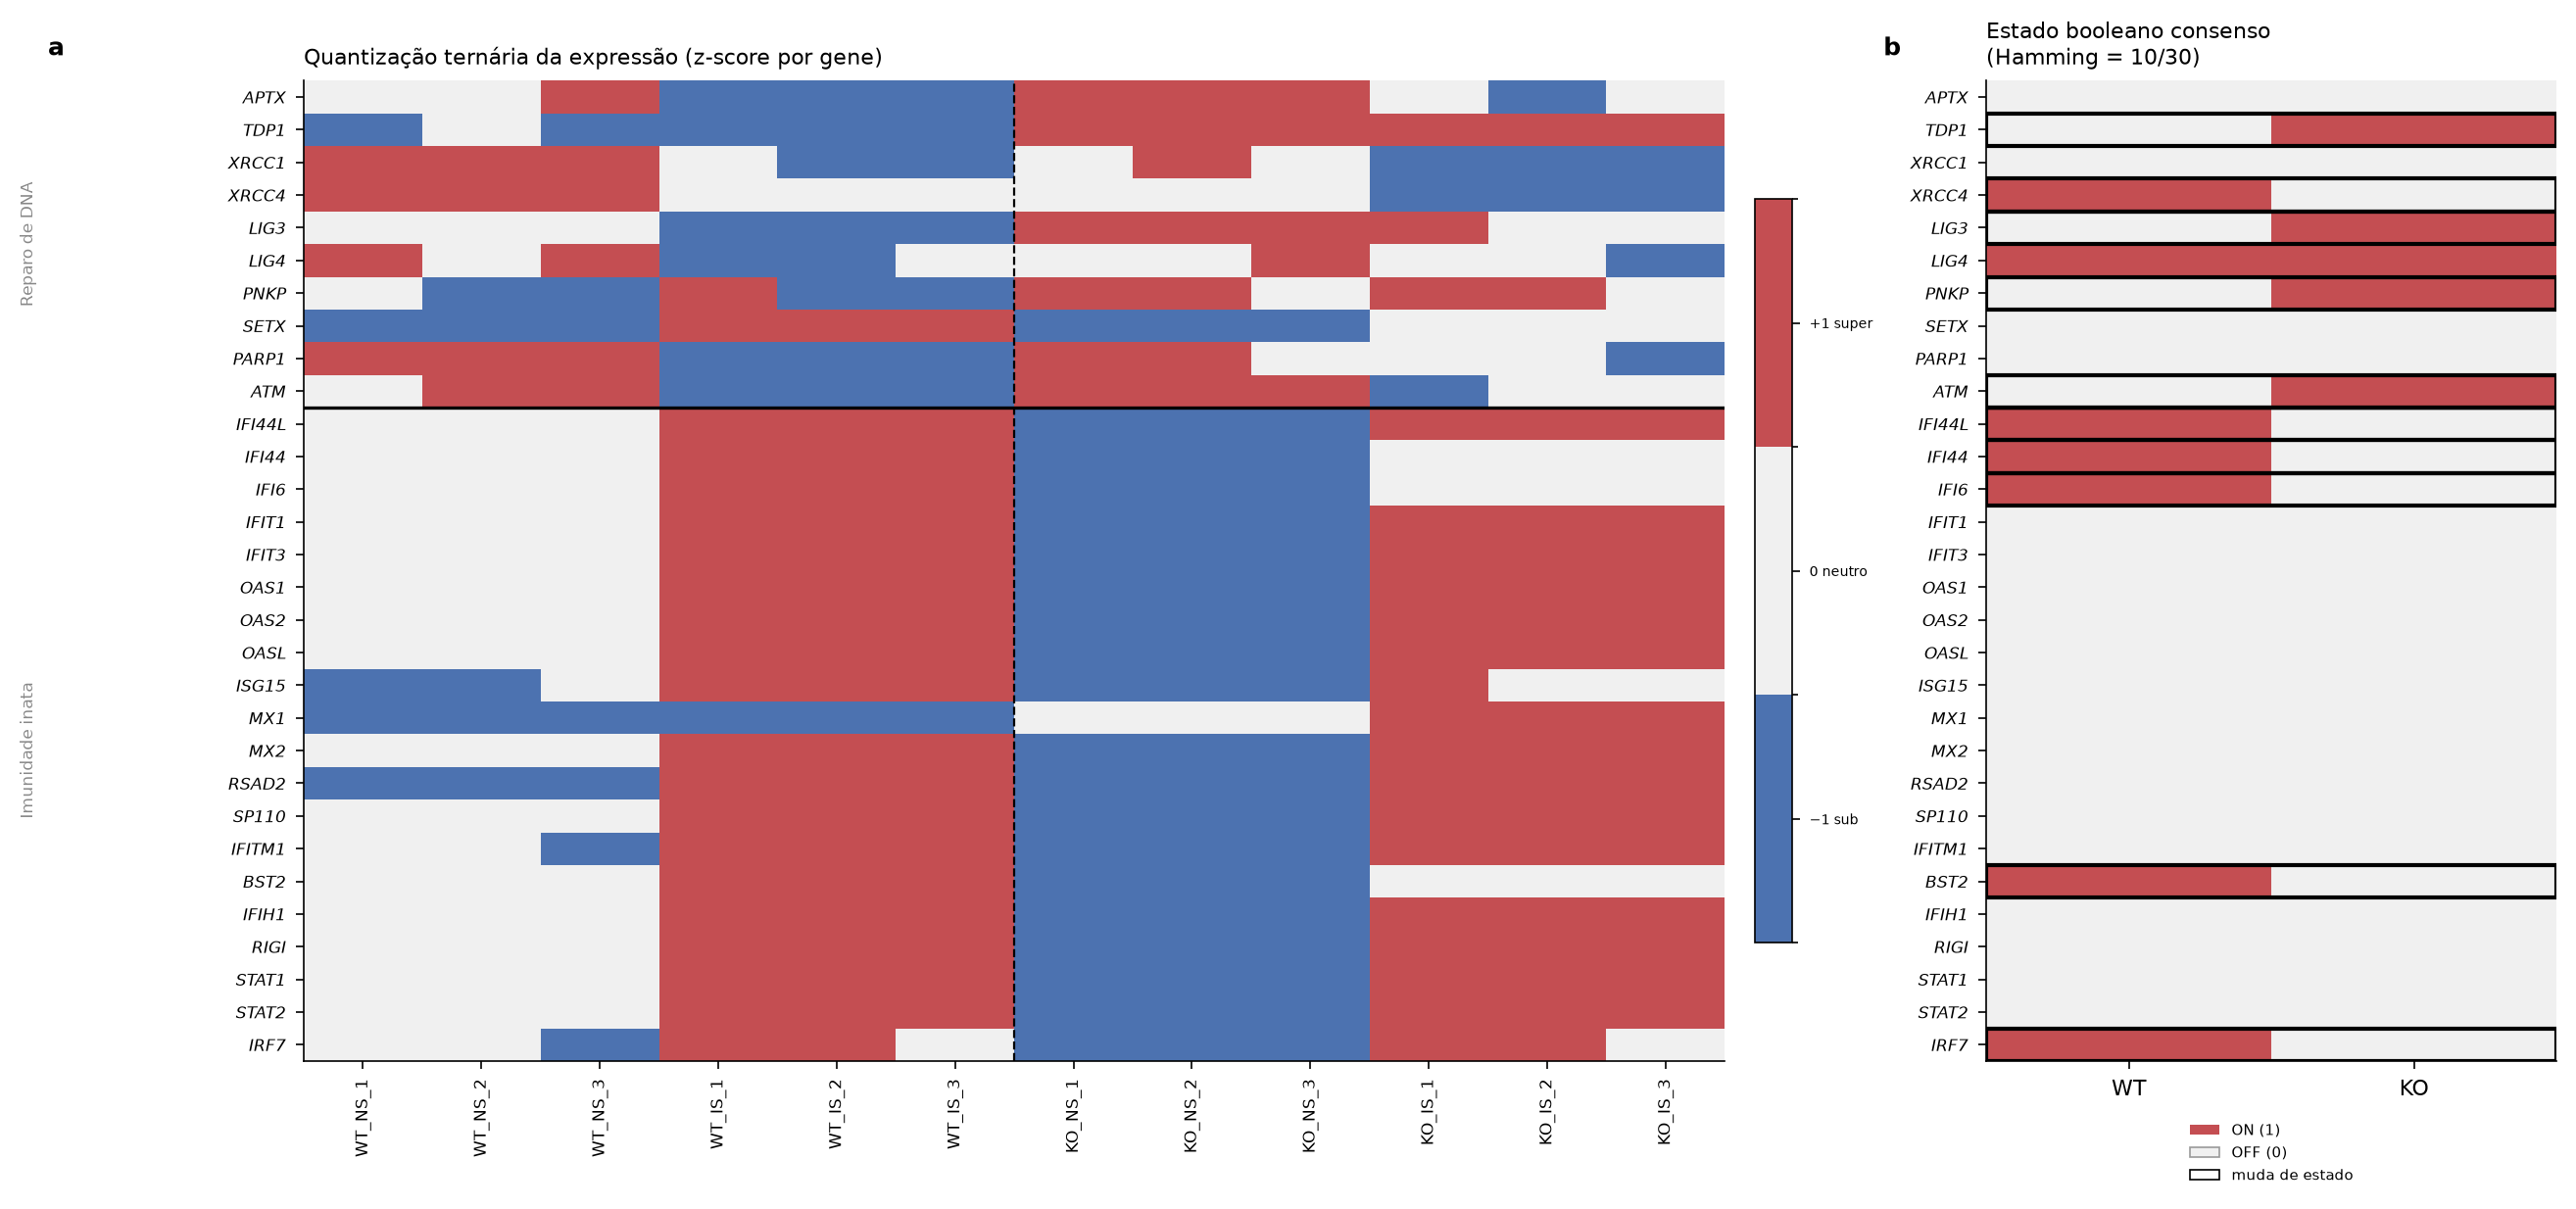
\includegraphics[width=\textwidth,height=0.80\textheight,keepaspectratio]{figure_discretizacao.png}
    \end{column}
    \begin{column}{0.40\textwidth}
      \small
      \begin{itemize}
        \item Painel de \textbf{30 genes} (reparo de DNA + imunidade), z-score por gene.
        \item \textbf{Quantização ternária} ($-1$/$0$/$+1$) e estado \textbf{booleano de consenso} por genótipo.
        \item \textbf{Distância de Hamming KO vs.\ WT $= 10/30$}: os 10 genes que mudam de estado misturam reparo (\gene{ATM}, \gene{TDP1}, \gene{LIG3}) e imunidade (\gene{IFI44L}, \gene{IFI6}, \gene{BST2}).
      \end{itemize}
    \end{column}
  \end{columns}
\end{frame}

% ---------- Slide 6: comparação de métodos ----------
\begin{frame}{Comparação de métodos - inferência de rede validada contra STRING}
  \begin{columns}[T]
    \begin{column}{0.58\textwidth}
      \centering
      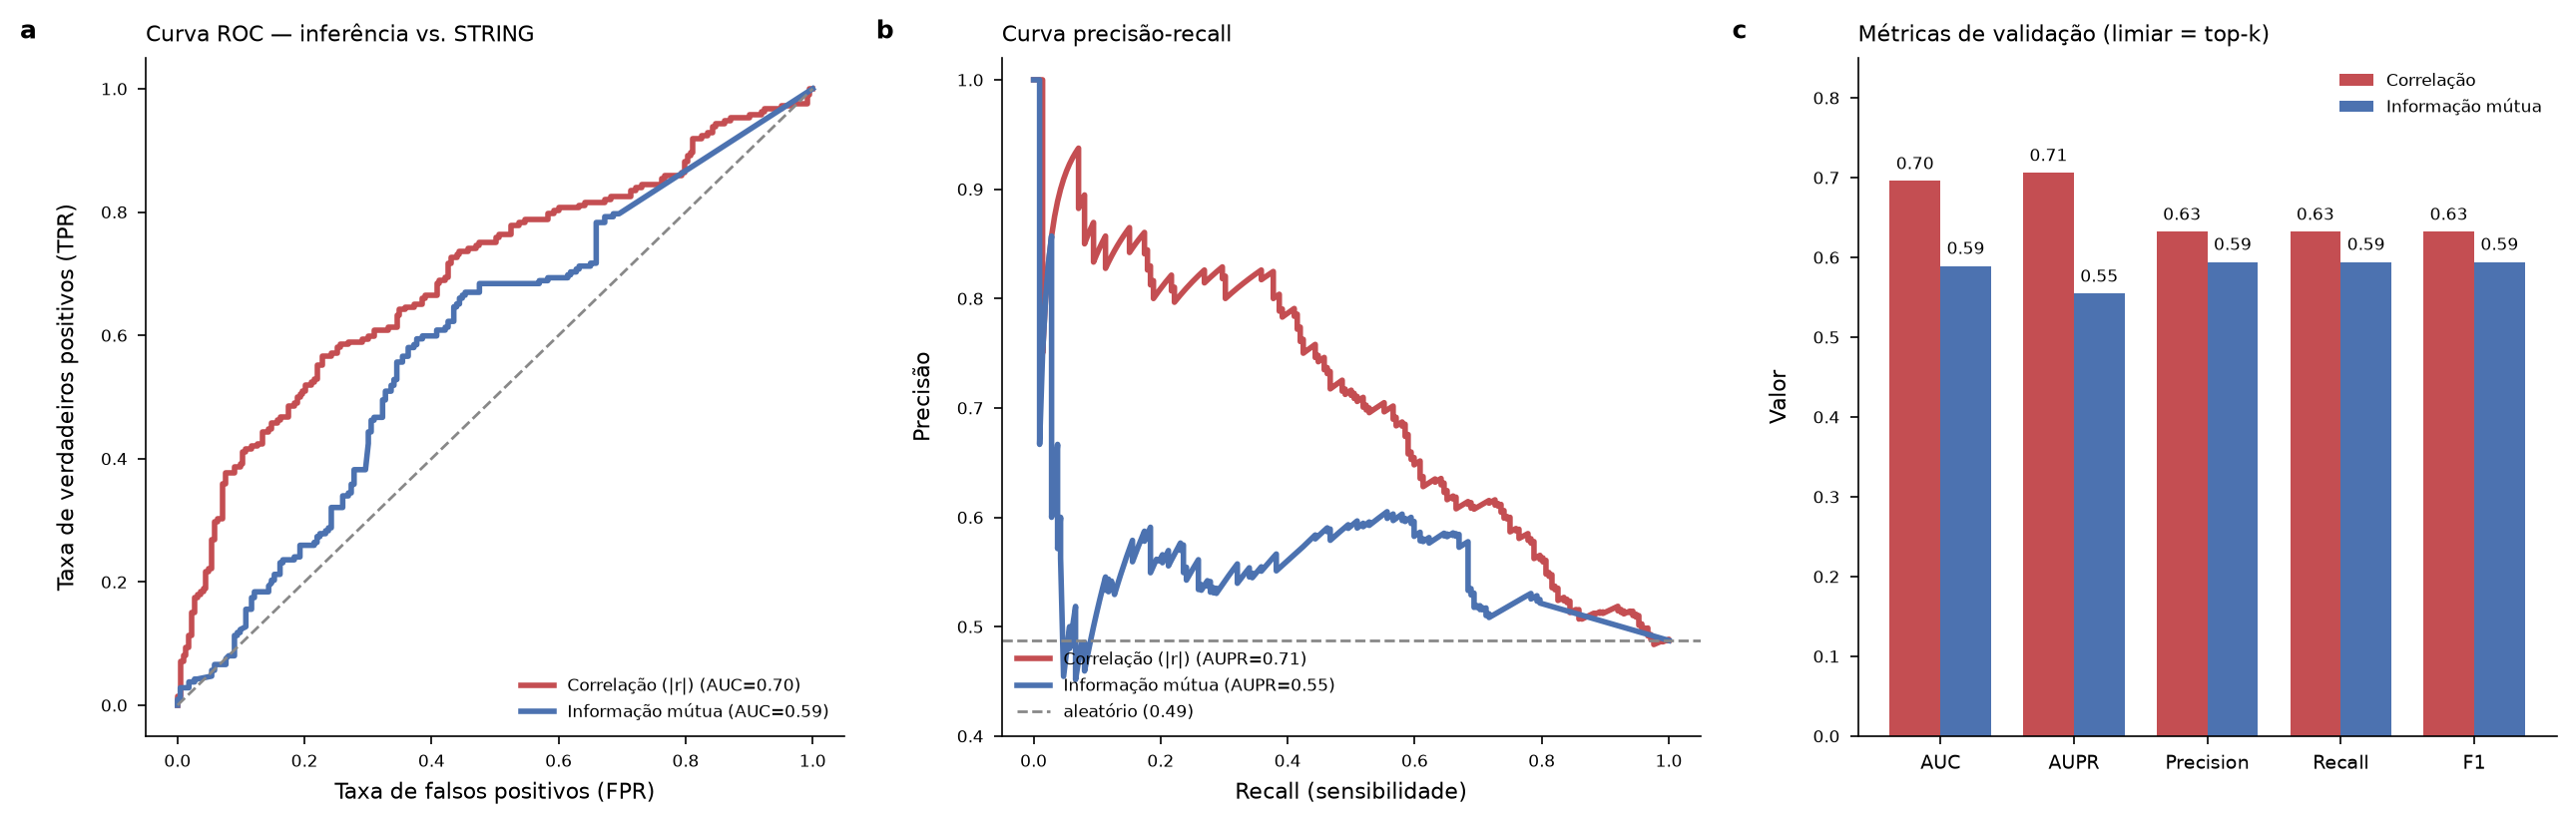
\includegraphics[width=\textwidth,height=0.62\textheight,keepaspectratio]{figure_grn_inference.png}
    \end{column}
    \begin{column}{0.42\textwidth}
      \scriptsize
      \begin{block}{Métricas (limiar top-$k$; gold $=$ STRING v12)}
        \begin{tabular}{lccc}
          \toprule
          Método & AUC & AUPR & F1 \\
          \midrule
          \textbf{Correlação} $|r|$ & \textbf{0,70} & \textbf{0,71} & \textbf{0,63} \\
          Informação mútua & 0,59 & 0,55 & 0,59 \\
          Aleatório & 0,50 & 0,49 & - \\
          \bottomrule
        \end{tabular}
      \end{block}
      \normalsize
      \begin{itemize}\small
        \item A \textbf{correlação supera a informação mútua} sob $M\ll N$ ($M=12$): estimadores de MI precisam de mais amostras.
        \item Resultado honesto: AUC$\approx$0,70 é o teto esperado ao inferir rede com $n=12$.
      \end{itemize}
    \end{column}
  \end{columns}
\end{frame}

% ---------- Slide 7: conclusões ----------
\begin{frame}{Conclusões}
  \begin{columns}[T]
    \begin{column}{0.5\textwidth}
      \textbf{\textcolor{aptxgreen}{Contribuições próprias}}
      \begin{itemize}\small
        \item Camada de Biologia de Sistemas sobre os dados: discretização, rede booleana e comparação de métodos de inferência com métricas.
        \item Teste de permutação que valida o classificador com $n$ pequeno.
      \end{itemize}
      \textbf{\textcolor{aptxblue}{Replicação/validação}}
      \begin{itemize}\small
        \item Confirma, de forma independente, a repressão do interferon no KO (Madsen et al., 2023).
      \end{itemize}
    \end{column}
    \begin{column}{0.5\textwidth}
      \textbf{Mensagem}
      \begin{block}{}
        \small A perda de \gene{APTX} é, transcricionalmente, um evento \textbf{imunológico}: o alarme antiviral basal depende de uma enzima de reparo de DNA.
      \end{block}
      \textbf{Limitações}
      \begin{itemize}\small
        \item $n=12$ limita a inferência causal de rede.
        \item Reanálise \emph{in silico}: sem validação experimental própria.
      \end{itemize}
      \vspace{0.4em}
      \centering\footnotesize\textcolor{aptxblue}{Código: github.com/ppufpr/projeto-APTX-AOA1}
    \end{column}
  \end{columns}
\end{frame}

\end{document}
